\documentclass[12pt,a4paper,english]{article}
\usepackage{times}
\usepackage[utf8]{inputenc}
\usepackage{babel,textcomp}
\usepackage{mathpazo}
\usepackage{mathtools}
\usepackage{amsmath,amssymb}
\usepackage{ dsfont }
\usepackage{listings}
\usepackage{graphicx}
\usepackage{float}
\usepackage{subfig} 
\usepackage[colorlinks]{hyperref}
\usepackage[usenames,dvipsnames,svgnames,table]{xcolor}
\usepackage{textcomp}
\definecolor{listinggray}{gray}{0.9}
\definecolor{lbcolor}{rgb}{0.9,0.9,0.9}
\lstset{backgroundcolor=\color{lbcolor},tabsize=4,rulecolor=,language=python,basicstyle=\scriptsize,upquote=true,aboveskip={1.5\baselineskip},columns=fixed,numbers=left,showstringspaces=false,extendedchars=true,breaklines=true,
prebreak=\raisebox{0ex}[0ex][0ex]{\ensuremath{\hookleftarrow}},frame=single,showtabs=false,showspaces=false,showstringspaces=false,identifierstyle=\ttfamily,keywordstyle=\color[rgb]{0,0,1},commentstyle=\color[rgb]{0.133,0.545,0.133},stringstyle=\color[rgb]{0.627,0.126,0.941},literate={å}{{\r a}}1 {Å}{{\r A}}1 {ø}{{\o}}1}

% Use for references
\usepackage[square,comma,numbers]{natbib}
%\DeclareRobustCommand{\citeext}[1]{\citeauthor{#1}~\cite{#1}}

% Fix spacing in tables and figures
%\usepackage[belowskip=0pt,aboveskip=5pt]{caption}
%\setlength{\intextsep}{10pt plus 2pt minus 2pt}

% Change the page layout
%\usepackage[showframe]{geometry}
\usepackage{layout}
\setlength{\hoffset}{-0.5in}  % Length left
\setlength{\voffset}{-0.8in}  % Length on top
\setlength{\textwidth}{470pt}  % Width /597pt
\setlength{\textheight}{670pt}  % Height /845pt
\setlength{\footskip}{25pt}

\newcommand{\VEV}[1]{\langle#1\rangle}
\title{FYS4150 - Project 4}
\date{}
\author{ Kristoffer Langstad\\ \textit{krilangs@uio.no}}

\begin{document}%layout
\maketitle
\begin{abstract}
In this project we want to find the phase transition at a critical temperature $T_C$ for a thermodynamic system with the Ising model in 2D from a ferromagnet phase to a paramagnet phase. This is a binary system where we look at the spins (up and down) for objects that interact only with its nearest neighbor at with different lattice sizes. We will use Monte Carlo and Metropolis algorithms develop the Ising model to solve the system numerically. Properties of the system are evaluated to find the number of Monte Carlo (MC) cycles needed to reach the system equilibrium. For a simple 2x2 lattice we have analytical values that we compare our numerics with. For this case we get best results as equal results within 4 leading digits for the mean energy and mean absolute magnetic moment with $10^7$ Monte Carlo cycles and $T=1.0$, while we get equal results within 3 leading digits for the specific heat and the susceptibility. Then for the evaluation of the 20x20 lattice for $T=1.0$ and $T=2.4$ with both an ordered and random initial spin orientation of the objects, we find that the system reaches the equilibrium state after around 8000 Monte Carlo cycles per lattice (which in this case represents time). For the random initial spins, the curves of the evaluated properties are much smoother and fluctuate less than the ordered. We also see that the higher temperature have a bigger affect on the values we evaluate than the lower temperature. We also find that the number of accepted configurations as a function of the temperature in the domain $T\in[1.0, 2.4]$ increase almost as an exponential with the temperature. For the probability distribution $P(E)$, which also is the number of times a given energy appears in the MC cycles, we see that the most probable energy for $T=1.0$ is more or less the ground state with energy -800. With increased temperature $T=2.4$, we get increased entropy and most likely energy around -490$\rightarrow$ -470. So a low energy is the same as the object has a low probability of jumping to the next state. For the evaluation of the Ising model near the critical temperature $T_C$ for lattices $L=[40,60,80,100]$, temperatures $T\in[2.15, 2.35]$, stepsize $\Delta T=0.002$ and MC cycles $5\cdot10^5$ we find the numerical critical temperature $T_C=2.268$ which indicate the phase transition. The analytical critical temperature is given as $T_C\approx2.269$ (\citet{PhysRev.65.117}), which compared to the numerical is equal with 2 leading digits. The critical temperature gets closer to the analytical in the thermodynamic limit $L\rightarrow\infty$.
\end{abstract}

\section{Introduction}
\label{sect:Introduction}
To study thermodynamics we can use statistical mechanics. A very popular method to do this is the Ising model. With this model we can simulate phase transitions for a magnetic system from a quantum mechanical perspective from a ferromagnet phase to a paramagnet phase. The model can then evaluate binary states for atomic spins (up and down) in a lattice of different sizes, where the spins only interact with its nearest neighbors. The phase transitions occur at a critical temperature from a system of a finite magnetic moment to a phase with zero magnetization.

In this project we will use the two-dimensional Ising model to find the phase transitions in a magnetic system for lattices of different sizes. For the lattices we have binary values as up and down. Since we use a 2D model, we have analytical values for the critical temperature which denotes the phase transitions. First we will evaluate a 2x2 lattice by using the Ising model and Monte Carlo and Metropolis algorithms to be used as benchmark calculations. Then we expand to a 20x20 lattice for various temperature values to evaluate the equilibrium time and the probability distribution of the energies. Then we study the phase transitions of the system to find the critical temperature. The numerical calculations are done in C++ with QT Creator on a Windows computer, while the plotting are done in Python 3.7.

In the methods section we look at the theory and execution of the physical problems and the numerical algorithms we are using. For the 2x2 lattice we calculate numerically known analytical values for expressions like the expectation values for the energy $E(T)$, mean absolute magnetic moment $|M(T)|$, specific heat $C_v(T)$ and susceptibility $\chi(T)$. Then we expand to a 20x20 lattice to see when the most likely state (equilibrium time) is reached with different temperatures. After the steady state is found, we find the probability distributions for the energies to have specific values. Then we evaluate for several lattice sizes $L=[40,60,80,100]$ to find the critical temperature of the system, which indicates the phase transition. In the results section we present and discuss the results we get from the numerical calculations. These results are also compared with analytical values for the 2x2 lattice case, and the analytical value for the critical temperature by \citet{PhysRev.65.117}. In the conclusion section, we present a conclusion to the project.

\section{Methods}
\label{sect:Methods}
\subsection{Ising Model Theory}
\label{subsect:Ising}
\subsection{Analytic Expressions}
\label{subsect:analytic}
\subsection{Numerical Algorithms}
\label{subsect:Algo}
\subsection{Equilibrium State}
\label{subsect:Equilibrium}
\subsection{Probability Distribution}
\label{subsect:Prob_dist}
\subsection{Phase Transitions}
\label{subsect:Phase_trans}
\subsection{Critical Temperature}
\label{subsect:TC}

\section{Results}
In the Data folder at the GitHub repository (\ref{sect:appendix}) we have text-files containing all the produced data to be evaluated either in tables or as plots. The corresponding plots can be found in the Figures folder.

For the first case with a $2x2$ lattice and with temperature $T=1.0 k_BT/J$ we calculated the expectation values numerically to compare with analytical values (calculated in section \ref{subsect:analytic}) as seen in Table \ref{tab:lattice_2} for some chosen number of Monte Carlo cycles. In the text file \textit{Lattice\_2x2} in the Data-folder at the GitHub repository \ref{sect:appendix} we see more values. In the mentioned table we see that our numerical values are within three leading digits after $10^6$ number of MC cycles for the energy and magnetization. For the specific heat and susceptibility we need $10^7$ MC cycles to get the same accuracy. For $10^8$ we see that the values start to get worse for some reason. 

\begin{table}[htbp]
	\centering
	%\hspace{-1cm}
	\begin{tabular}{ |c|c|c|c|c| }
		\hline \rule{0pt}{13pt}
		 & Analytical & MC=$10^6$ & MC=$10^7$ & MC=$10^8$\\
		\hline \rule{0pt}{13pt}
		$\langle E(T)\rangle$ & -7.9839283 & -7.9837760 & -7.9839400 & -7.9841136 \\
		\hline \rule{0pt}{13pt}
		$\langle |M(T)|\rangle$ & 3.9946429 & 3.9947200 & 3.9946598 & 3.9947162 \\
		\hline \rule{0pt}{13pt}
		$C_V(T)$ & 0.12832933 & 0.12952878 & 0.12823488 & 0.12684906 \\
		\hline \rule{0pt}{13pt}
		$\chi(T)$ & 0.016042958 & 0.015428122 & 0.015953482 & 0.015789361 \\
		\hline 
	\end{tabular}	
	\caption{Table for the mean energy $E$, mean absolute magnetic moment $|M|$, specific heat $C_V$ and susceptibility $\chi$ for both analytical and numerical values for a $2x2$ lattice and $T=1.0 k_BT/J$. Here we see that after $10^6$ Monte Carlo cycles, the numerical values get quite close to the analytical values. We get the best values for $10^7$ MC cycles, since with $10^8$ cycles the values start to get worse again.}
	\label{tab:lattice_2}
\end{table}

Then we wanted to find when the most likely state was reached. To do this we used a $20x20$ lattice for $T=1.0$ and $T=2.4$. We also calculated for a case with ordered initial spin orientation, and for a case with random initial spin orientation. We evaluated the expectation values for the energy, magnetization and the total number of accepted configurations as functions of the number of MC cycles (sweeps per lattice) representing time. For the number of accepted configurations, we also plotted it as function of the temperature. 

In Figure \ref{fig:equil_E} we have three plots of the expectation values for the energy for ordered (fig. \ref{fig:Ordered_E1} and \ref{fig:Ordered_E2}) and random (fig. \ref{fig:Random_E}) initial spin orientation for $T=1.0$ and $T=2.4$. From these plots we see that the expectation energies are higher for the higher temperature. This makes sense since increasing the temperature also increases the entropy of the system, which then increases the energy of the system. By comparing the ordered and random initial spins, we see that the random spins reaches the equilibrium state much earlier than for ordered spin. For the random spin the energy values also decrease with number of MC cycles, while for ordered spin the energies increase with number of MC cycles. For the lower temperature the system also seems to reach the equilibrium state a little earlier than for the higher temperature.

In Figure \ref{fig:equil_M} we have three plots of the expectation values for the absolute magnetization for ordered (fig. \ref{fig:Ordered_M1} and \ref{fig:Ordered_M2}) and random (fig. \ref{fig:Random_M}) initial spin orientation for $T=1.0$ and $T=2.4$. From Figure \ref{fig:Ordered_M1} we see that the magnetization values does not change much and reaches equilibrium state around 7000 MC cycles. From Figure \ref{fig:Ordered_M2} we see that the values drops much more before reaching the equilibrium state around 8000 MC cycles. For the random spins in Figure \ref{fig:Random_M} the curve for lower $T$ reaches equilibrium state much earlier at around 4000MC cycles, while for higher $T$ it reaches equilibrium state around 8000 MC cycles. These expectation figures behaves like the opposite as the energies in Figure \ref{fig:equil_E}. So when the expectations energy of the system increases, the expectation values of the magnetization decreases. We also see that for lower temperature, the system seem to be more stable since it reaches the equilibrium state earlier. From these two figures we can conclude that the system reaches the equilibrium state earliest around 8000 MC cycles, so to be safe we can say that the equilibrium state has been reached after 9000 MC cycles.

In Figure \ref{fig:equil_Nconfigs} we have three plots for the total number of accepted configurations for ordered (fig. \ref{fig:Ordered_Nconfigs1} and \ref{fig:Ordered_Nconfigs2}) and random (fig. \ref{fig:Random_Nconfigs}) initial spin orientation for $T=1.0$ and $T=2.4$. These figures behave the same way like the expected energy of the system. So there is a connection between the energy and the number of accepted configurations. This also applies to the temperature of the system, where the number of accepted configurations increase much more for higher temperature for ordered initial spins. For the random initial spin the total number of configurations decrease much more for lower temperature, and seem to be much more stable than the rest. In Figure \ref{fig:acceptvsT} we see the temperature dependence on the total number of accepted configurations. The number of accepted configurations increases close to an exponential as the temperature increases.

For the probability distribution $P(E)$ for the $L=20$ lattice and $4\cdot10^4$ MC cycles, we counted the number of times a given energy appears in the MC cycles for $T=1.0$ (fig. \ref{fig:Prob1}) and $T=2.4$ (fig. \ref{fig:Prob2}). Since we found that the system reach the equilibrium state after around 9000 MC cycles, we start to count the probability distribution after this. For the low temperature $T=1.0$ the most probable energy is the ground state energy -800. This means that the probability of an object in the system to jump to the next state is very low. For the higher temperature $T=2.4$, the most probable energy is around -470. This probability has a standard deviation of $\sigma_E=3.04$ and variance $\sigma_E^2=9.27$. So now the probability of an object to jump to the next state is much higher since the entropy of the system is higher.. This probability distribution is similar to a Gaussian distribution. This distribution has a higher standard deviation of $\sigma_E=56.62$ and variance $\sigma_E^2=3206$.

To study the phase transition of the system with the two-dimensional Ising model near the critical temperature $T_C$, we calculated the expectation values for $\langle E(T)\rangle$ (fig. \ref{fig:Phase_E}) and $\langle |M(T)|\rangle$ (fig. \ref{fig:Phase_M}), the heat capacity $C_V(T)$ (fig. \ref{fig:Phase_CV}) and the susceptibility $\chi(T)$ (fig. \ref{fig:Phase_Xi}) for lattices $L=[40,60,80,100]$, temperatures $T\in[2.15,2.35]$, $\Delta T=0.002$ and $5\cdot10^5$ MC cycles. The phase transition plots can be seen in Figure \ref{fig:Phases}. In the phase plot for the magnetization, we see that as $L\rightarrow\infty$ the corresponding curves converges. This convergence point is the critical temperature which from \citet{PhysRev.65.117} is given as an analytical value as $T_C\approx2.269$. The phase transition is where the critical temperature is. This is also indicated where the heat capacity and susceptibility has their maximum \cite{ComPhys}\footnote{Chapter 13.4: Phase Transitions and Critical Phenomena}. The phase before the transition is the ferromagnetic phase, while the phase after is the paramagnetic phase. In the paramagnetic phase we see that the magnetization drops towards zero. For the energy we see that in the paramagnetic phase, the energy increases more and more as $L\rightarrow\infty$. For the heat capacity and the susceptibility, the curves gets a higher and higher maximum peak as $L\rightarrow\infty$.

In Figure \ref{fig:TC} we see the phase transition plot for the heat capacity again, but now we have plotted the critical temperatures for each lattice and the analytic critical temperature by \citet{PhysRev.65.117} ($T_C\approx2.269$). In Table \ref{tab:TC} we see the critical temperatures for the lattices and the analytical $T_C$. As $L\rightarrow\infty$ we see that the critical temperature converges to the analytical $T_C$. 

\begin{table}[htbp]
	\centering
	%\hspace{-1cm}
	\begin{tabular}{ |c|c| }
		\hline \rule{0pt}{13pt}
		Lattice & $T_C$ \\
		\hline \rule{0pt}{13pt}
		$40x40$ & 2.282 \\
		\hline \rule{0pt}{13pt}
		$60x60$ & 2.276 \\
		\hline \rule{0pt}{13pt}
		$80x80$ & 2.274 \\
		\hline \rule{0pt}{13pt}
		$100x100$ & 2.268 \\
		\hline \rule{0pt}{13pt}
		Analytic & 2.269 \\
		\hline 
	\end{tabular}	
	\caption{Table for the calculated critical temperatures for the lattices for the specific heat of the system. As $L\rightarrow\infty$ we see that the calculated critical temperature converges to the analytic.}
	\label{tab:TC}
\end{table}

\begin{figure}[htbp]
	%\hspace*{-2.5cm}
	\subfloat[Expectation values for the energy with ordered initial spin orientation and $T=1.0$. Here it looks like the system reaches an equilibrium state after around 7000 MC cycles. The energies are also very close to the ground state energy. \label{fig:Ordered_E1} ]{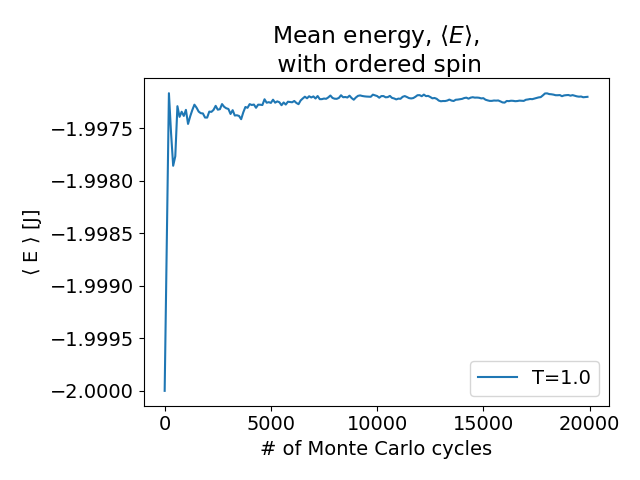
\includegraphics[width=0.5\linewidth]{E_Ordered_1.png}}
	\hspace{0.5em}
	\subfloat[Expectation values for the energy with ordered initial spin orientation and $T=2.4$. Here it looks like the system reaches an equilibrium state after around 8000 MC cycles. In this case the energies are much higher than for the lower $T$ since the entropy of the system has increased with the increased $T$ value. \label{fig:Ordered_E2} ]{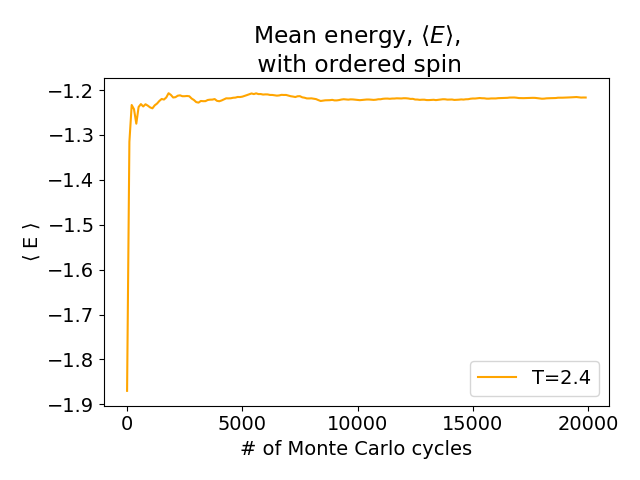
\includegraphics[width=0.5\linewidth]{E_Ordered_2_4.png}}\\
	\subfloat[Expectation values for the energy with random initial spin orientation and both temperatures. Here it looks like the system reaches an equilibrium state after around 4000 MC cycles for $T=1.0$. For $T=2.4$ it looks like the system reach equilibrium around 5000 MC cycles. \label{fig:Random_E}]{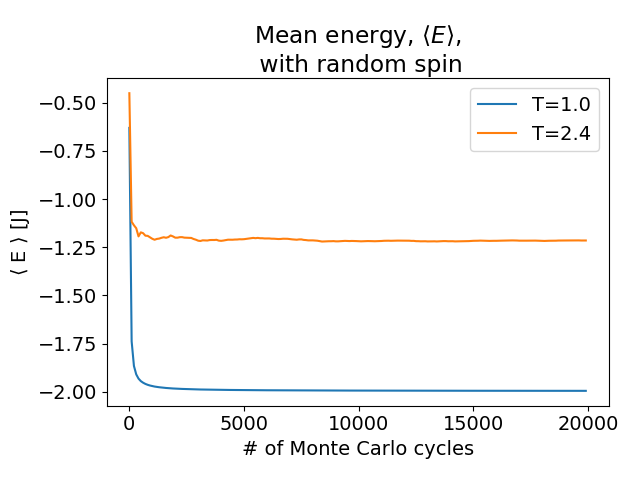
\includegraphics[width=0.6\linewidth]{E_Random.png}}
	\caption{Here we have plots for the expectation values for the energy splitted into one for ordered initial spin orientation and $T=1.0$, one for ordered initial spin orientation and $T=2.4$ and one for random initial spin orientation for both temperatures. Here we see that with random initial spin the system reaches the equilibrium state much earlier than for the ordered spin. The energies for higher $T$ value are much higher than for lower $T$.\label{fig:equil_E}}
\end{figure}

\begin{figure}[htbp]
	%\hspace*{-2.5cm}
	\subfloat[Expectation values for the absolute magnetization with ordered initial spin orientation and $T=1.0$. Here it looks like the system reaches an equilibrium state after around 7000 MC cycles. The magnetization values changes very little. \label{fig:Ordered_M1} ]{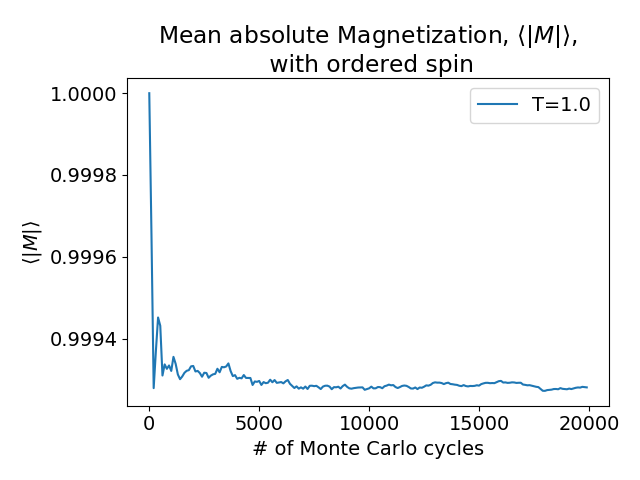
\includegraphics[width=0.5\linewidth]{M_Ordered_1.png}}
	\hspace{0.5em}
	\subfloat[Expectation values for the absolute magnetization with ordered initial spin orientation and $T=2.4$. Here it looks like the system reaches an equilibrium state after around 8000 MC cycles. In this case the magnetization values are much lower than for the lower $T$. \label{fig:Ordered_M2} ]{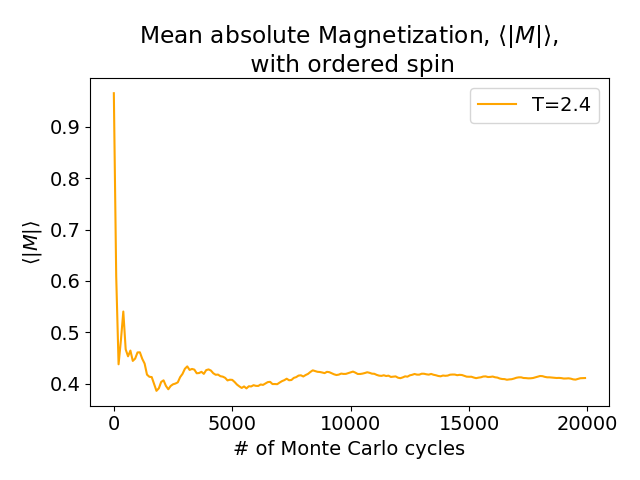
\includegraphics[width=0.5\linewidth]{M_Ordered_2_4.png}}\\
	\subfloat[Expectation values for the absolute magnetization with random initial spin orientation and both temperatures. Here it looks like the system reaches an equilibrium state after around 4000 MC cycles for $T=1.0$. For $T=2.4$ it looks like the system reach equilibrium around 8000 MC cycles. \label{fig:Random_M}]{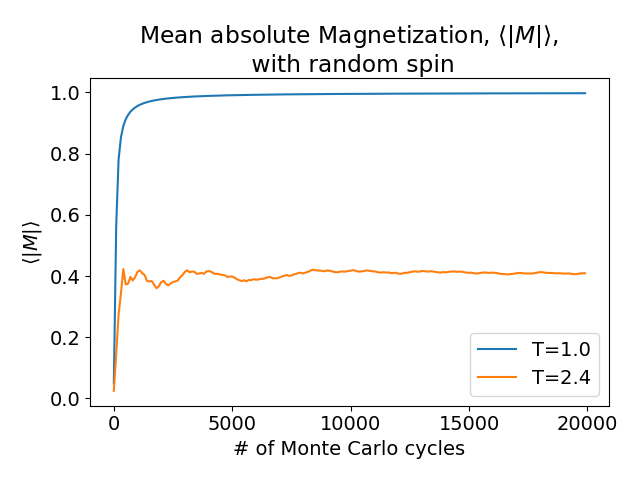
\includegraphics[width=0.6\linewidth]{M_Random.png}}
	\caption{Here we have plots for the expectation values for the absolute magnetization splitted into one for ordered initial spin orientation and $T=1.0$, one for ordered initial spin orientation and $T=2.4$ and one for random initial spin orientation for both temperatures. Here we see that with random initial spin the system reaches the equilibrium state much earlier than for the ordered spin. The energies for higher $T$ value are much higher than for lower $T$.\label{fig:equil_M}}
\end{figure}

\begin{figure}[htbp]
	%\hspace*{-2.5cm}
	\subfloat[Total number of accepted configurations normalized as function of the number of MC cycles with ordered initial spin orientation and $T=1.0$. The number of accepted config values changes very little, and is very low. \label{fig:Ordered_Nconfigs1} ]{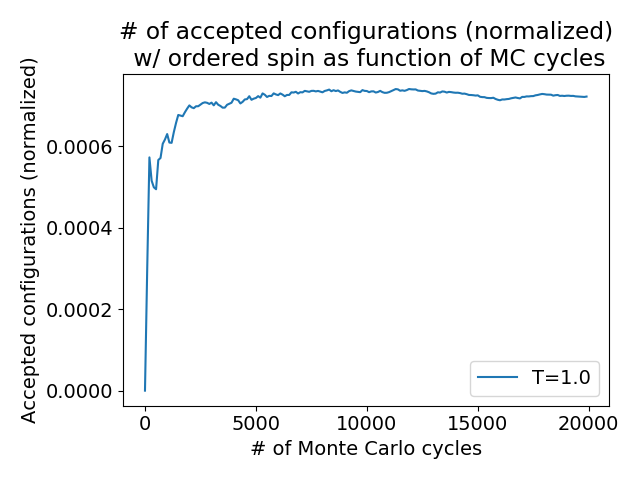
\includegraphics[width=0.5\linewidth]{Accpt_Ordered_1.png}}
	\hspace{0.5em}
	\subfloat[Total number of accepted configurations normalized as function of the number of MC cycles with ordered initial spin orientation and $T=2.4$. In this case the number of accepted configs are much higher than for the lower $T$. \label{fig:Ordered_Nconfigs2} ]{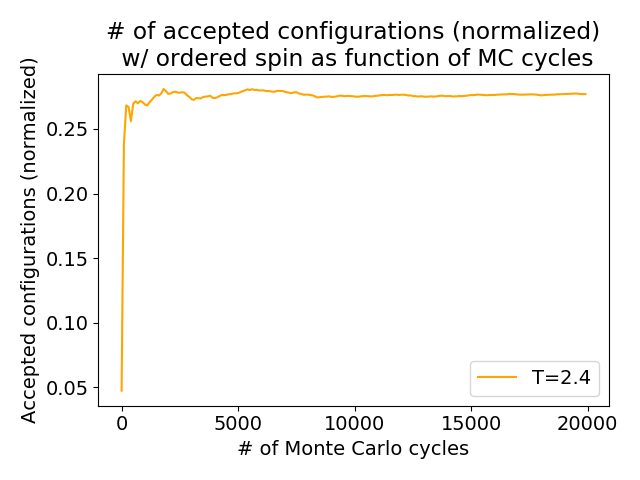
\includegraphics[width=0.5\linewidth]{Accpt_Ordered_2_4.png}}\\
	\subfloat[Total number of accepted configurations normalized as function of the number of MC cycles with random initial spin orientation and both temperatures. \label{fig:Random_Nconfigs}]{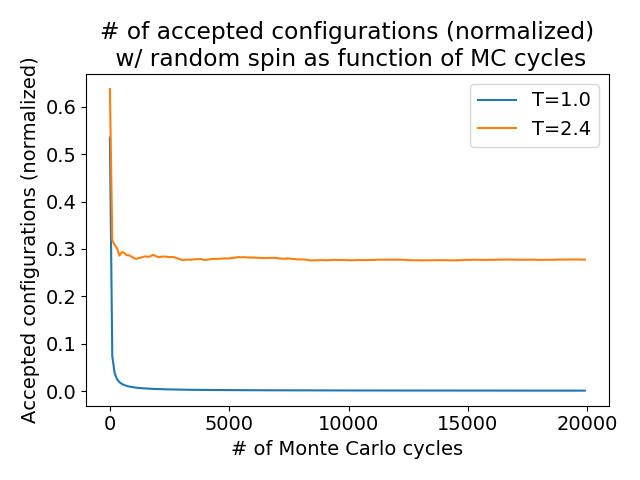
\includegraphics[width=0.6\linewidth]{Accpt_Random.png}}
	\caption{Here we have plots for the total number of accepted configurations normalized as function of the number of MC cycles splitted into one for ordered initial spin orientation and $T=1.0$, one for ordered initial spin orientation and $T=2.4$ and one for random initial spin orientation for both temperatures. Here we see that with random initial spin the system reaches the equilibrium state much earlier than for the ordered spin. The number of accepted configurations are much higher for higher $T$. The curves behave like for the energy curves in Figure \ref{fig:equil_E}. So there is a connections between the expected energy of the system and the number of accepted configurations.\label{fig:equil_Nconfigs}}
\end{figure}

\begin{figure}[htbp]
	\centering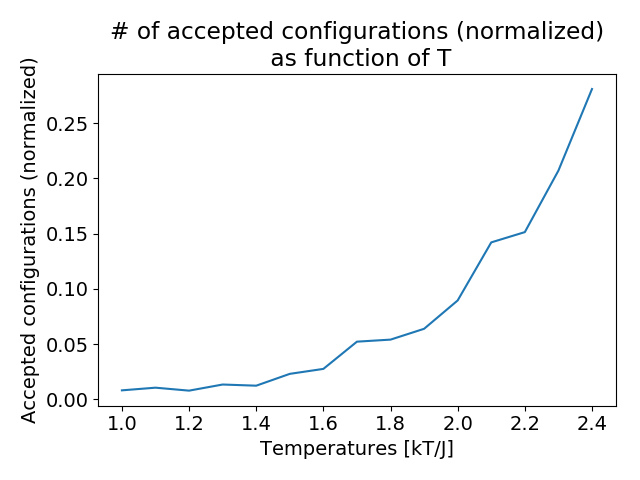
\includegraphics[width=0.6\linewidth]{AccptVsT.png}
	\caption{Figure for the number of accepted configurations normalized as function of the temperature. Here we see that the number of accepted configurations increase almost exponentially as the temperature increase. \label{fig:acceptvsT}}
\end{figure}

\begin{figure}[htbp]
	%\hspace*{-2.5cm}
	\subfloat[Probability distribution for $T=1.0$ as function of the energy. Here almost all the counted energies are the ground state energy at -800. So the most probable energy of the system is the ground state energy. This means that there is a low probability of the object to jump to the next state. \label{fig:Prob1} ]{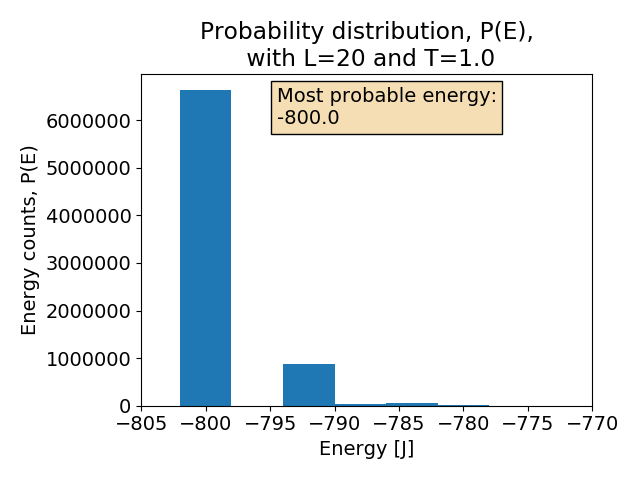
\includegraphics[width=0.5\linewidth]{Prob_1.png}}
	\hspace{0.5em}
	\subfloat[Probability distribution for $T=2.4$ as function of the energy. Here the energies are more distributed around the most probable energy of around -470. The curve looks like a Gaussian. The given most probable energy in the figure is the highest number of counted energy. \label{fig:Prob2} ]{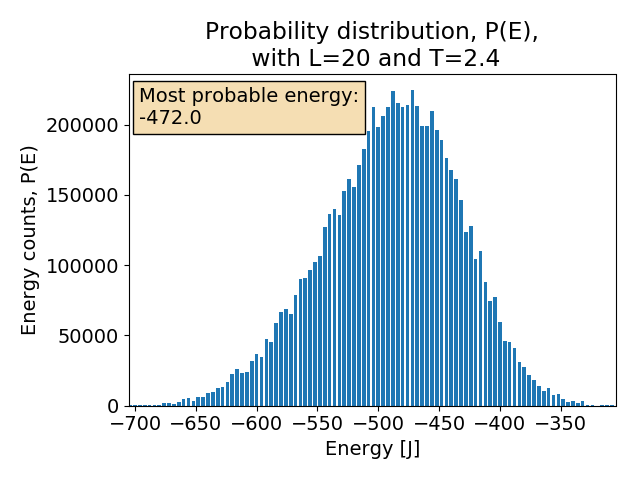
\includegraphics[width=0.5\linewidth]{Prob_2_4.png}}
	\caption{Figures for the probability distributions $P(E)$ as the number of times a given energy appears in the MC cycles fro $T=1.0$ (fig. \ref{fig:Prob1}) and $T=2.4$ (fig. \ref{fig:Prob2}).\label{fig:}}
\end{figure}

\begin{figure}[htbp]
	%\hspace*{-2.5cm}
	\subfloat[Phase plot for the expectation values for the energy $\langle E(T)\rangle$. \label{fig:Phase_E} ]{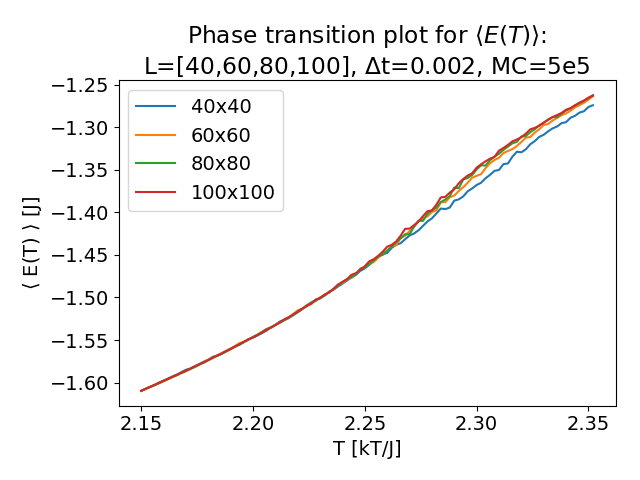
\includegraphics[width=0.5\linewidth]{Phase_E(T).png}}
	\hspace{0.5em}
	\subfloat[Phase plot for the expectation values for the absolute magnetization $\langle |M(T)|\rangle$. \label{fig:Phase_M} ]{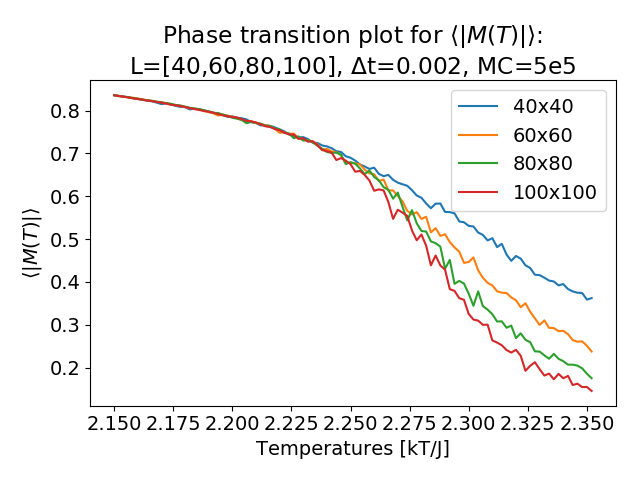
\includegraphics[width=0.5\linewidth]{Phase_M(T).png}}\\
	\subfloat[Phase plot for the heat capacity $C_V(T)$. \label{fig:Phase_CV}]{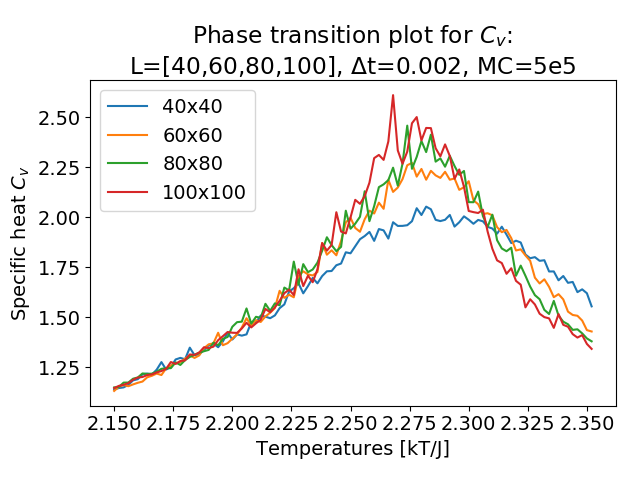
\includegraphics[width=0.5\linewidth]{Phase_Cv(T).png}}
	\hspace{0.5em}
	\subfloat[Phase plot for the susceptibility $\chi(T)$. \label{fig:Phase_Xi}]{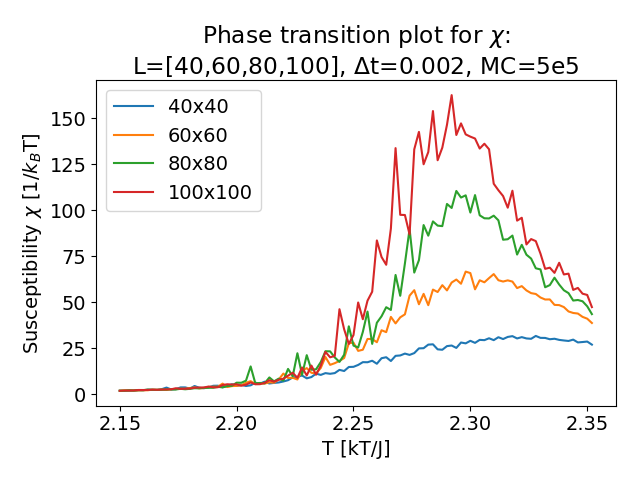
\includegraphics[width=0.5\linewidth]{Phase_Xi(T).png}}
	\caption{Here we see phase plots for the expectation values of the energy and absolute magnetization, the heat capacity and the susceptibility for lattices $L=[40,60,80,100]$, temperatures $T\in[2.15,2.35]$, $\Delta T=0.002$ and $5\cdot10^5$ MC cycles near the critical temperature $T_C$. The phase transition is indicated where the heat capacity and susceptibility has their maximum, called the critical point (ch. 13.4 in \citet{ComPhys}).\label{fig:Phases}}
\end{figure}

\begin{figure}[htbp]
	\centering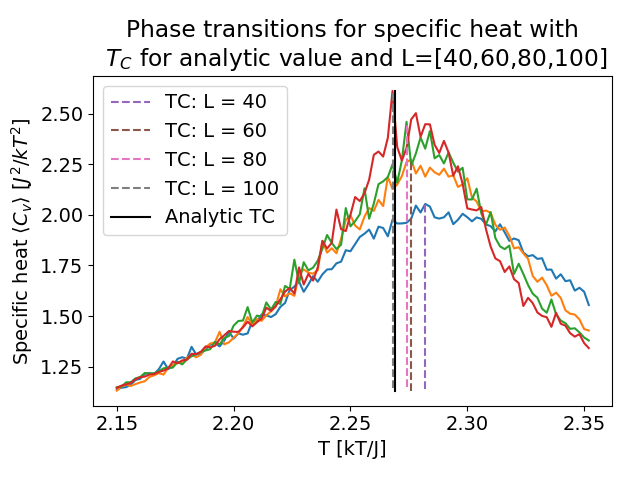
\includegraphics[width=0.7\linewidth]{CV_TC.png}
	\caption{Figure for the heat capacity where the dotted straight lines indicate the individual critical temperatures for the lattices, while the black straight line indicates the analytic critical temperature from \citet{PhysRev.65.117}. We see that as $L\rightarrow\infty$, the lattice critical temperature converges towards the analytic critical temperature. \label{fig:TC}}
\end{figure}

\section{Conclusion}
In this project we have simulated a phase transition for a binary magnetic system by using the Ising model in 2D for a ferromagnetic phase to a paramagnetic phase with zero magnetization. We have used Monte Carlo and Metropolis algorithms with the Ising model to simulate the phase transition for different sizes of lattices for objects with either spin up or down.

We have calculated expectation values for a 2x2 lattice which we have compared with analytic values. For $10^7$ MC cycles we got equal results with at least three leading digits for all the expectation values we calculated. For the next case with a 20x20 lattice with both ordered and random initial spin orientation, we found that the system reaches a equilibrium state after around 9000 MC cycles. This threshold was then used as a mark to start calculating the probability distribution $P(E)$, where we ran with $4\cdot10^4$ MC cycles, by counting the number of times a given energy appeared in the MC cycles. For the lower temperature we got that the most probable energy is the ground state energy, such that an object hos a very low chance of not being in the ground state. For higher temperature, the probability of jumping states increases. For an increase in the temperature of the system, this lead to an increase in the energy and in the number of accepted configurations. This also lead to the magnetization going towards zero, as wanted. For the phase transition and critical temperature, we tested for lattice sizes $L\rightarrow\infty$ for $L=[40,60,80,100]$. Here we found the critical temperature by looking at the maximum of the heat capacity for the lattices. To do this we needed enough MC cycles to get enough data. So for $5\cdot10^5$ MC cycles, $\Delta T=0.002$, $T\in[2.15,2.35]$ and $L=100$ (ideally want $L\rightarrow\infty$), we got a critical temperature $T_C=2.268$. This is close to the analytical $T_C\approx2.269$ found by \citet{PhysRev.65.117}. In this limit at $T_C$, the system goes from a ferromagnetic phase to a paramagnetic phase.

For even better results we could be to run for larger lattice $L$ sizes, use smaller $\Delta T$ values and/or even more MC cycles. The most efficient would probably be to use more MC cycles to produce more data. By looking at the phase transition plots in Figure \ref{fig:Phases}, we see that the curves are not optimal since they are not smooth. This comes from that we have not used enough MC cycles, but they are good enough as seen when comparing the critical temperatures. The CPU time for running $5\cdot10^5$ MC cycles was around 16,5 hours. So to increase the MC cycles more, would increase the CPU time by a lot. This could be done with more time. The reason for this long time, is that the code was not properly parallelized. For some reason, the armadillo library and openMP library made an error on the used Windows computer. This error came when implementing the compiler flag \textit{-fopenmp}. Without the mentioned compiler flag, the parallelization would not be initialized. With the flag, then some of the armadillo functions would not work properly. With more time, this error could most likely have been fixed. So by parallelizing the code, the CPU time would go down drastically.

\appendix
\section{Appendix}
\label{sect:appendix}
Link to GitHub repository:\\
\url{https://github.com/krilangs/FYS4150/tree/master/Project4}

\bibliographystyle{plainnat}
\bibliography{myrefs}
\end{document}